\documentclass{article}

\usepackage{booktabs}
\usepackage{tabularx}
\usepackage{hyperref}
\usepackage{amsmath, mathtools}
\usepackage{amsfonts}
\usepackage{amssymb}
\usepackage{graphicx}
\usepackage{colortbl}
\usepackage{xr}
\usepackage{hyperref}
\usepackage{longtable}
\usepackage{xfrac}
\usepackage{tabularx}
\usepackage{booktabs}
\usepackage{graphicx}
\usepackage{float}
\usepackage{siunitx}
\usepackage{caption}
\usepackage{pdflscape}
\usepackage{afterpage}
\usepackage{fullpage}
\usepackage{titlesec}
\usepackage[shortlabels]{enumitem}
\usepackage[round]{natbib}
\usepackage{array}
\usepackage{geometry}

\hypersetup{
    colorlinks=true,       % false: boxed links; true: colored links
    linkcolor=red,          % color of internal links (change box color with linkbordercolor)
    citecolor=green,        % color of links to bibliography
    filecolor=magenta,      % color of file links
    urlcolor=cyan           % color of external links
}

\title{Hazard Analysis\\\progname}

\author{\authname}

\date{}

\input{../Comments}
%% Common Parts

\newcommand{\progname}{Chess Connect} % PUT YOUR PROGRAM NAME HERE
\newcommand{\authname}{Team \#4,
\\ Alexander Van Kralingen
\\ Arshdeep Aujla
\\ Jonathan Cels
\\ Joshua Chapman
\\ Rupinder Nagra} % AUTHOR NAMES without MacIDs 

\usepackage{hyperref}
    \hypersetup{colorlinks=true, linkcolor=blue, citecolor=blue, filecolor=blue,
                urlcolor=blue, unicode=false}
    \urlstyle{same}

\newcommand{\projectoverview}{

The Chess Connect project allows two users to play a game of chess on a physical board with the information being transmitted to an online web application over Bluetooth.
Currently, there is no way for players to seamlessly switch between playing on a physical board and playing online, but Chess Connect intends to change this by creating a central platform that will provide flexibility and remove barriers for new players looking to learn the game.

}

\begin{document}

\maketitle
\thispagestyle{empty}

~\newpage

\pagenumbering{roman}

\begin{table}[hp]
\caption{Revision History} \label{TblRevisionHistory}
\begin{tabularx}{\textwidth}{llX}
\toprule
\textbf{Date} & \textbf{Developer(s)} & \textbf{Change}\\
\midrule
2022-10-09 & Arshdeep Aujla & Added table for FMEA\\
2022-10-09 & Alexander Van Kralingen & Updated Introduction, Scope, System Boundaries and Critical Assumptions\\
2022-10-09 & Alexander Van Kralingen & Fixed FMEA table placement\\
2022-10-19 & Jonathan Cels & Added requirements\\
2022-10-19 & Joshua Chapman & FMEA table edits and description changed\\
2022-10-19 & Rupinder Nagra & Added roadmap\\
2023-04-04 & Alexander Van Kralingen & Addressed peer review issues and TA feedback\\
\bottomrule
\end{tabularx}
\end{table}

~\newpage

\tableofcontents

~\newpage

\pagenumbering{arabic}

\section{List of Tables}
\begin{itemize}
    \item \textbf{Table 1:} Failure Mode and Effects Analysis
\end{itemize}

\section{List of Figures}
\begin{itemize}
    \item \textbf{Figure 1:} Overall System Context
\end{itemize}

\section{Introduction}{
    Creating a product designed for consumer use requires a robust hazard identification and mitigation strategy before the 
    product is released to the public. A hazard can be defined as any source of potential damage, harm or adverse health effects 
    on something or someone \cite{CCOHS}. A hazard for the \progname{} system is anyhting that could either harm the user or cause system failure.
}

\section{Project Overview}
\projectoverview

\section{Scope and Purpose of Hazard Analysis}{
    In this document, the potential cause for hazards will be explored in detail, as well as methods for preemptive detection, 
    and recommended actions should the hazard still present itself. Its purpose is to identify potential sources for harm or 
    failure and address them before they are presented in the finished product.
}

\section{System Boundaries and Components}{
    The \progname{} system is comprised of three main components:
    \begin{enumerate}
        \item The hardware including the chess pieces, board, microcontroller and all electronic components:
        \begin{itemize}
            \item LEDs
            \item Hall-Effect sensors
            \item LCD screen
            \item Connecting wires
            \item Power adapter
        \end{itemize}
        \item The nearby server to recieve data through a Bluetooth connection.
        \item The hosted Web Application used to connect to the game remotely.
    \end{enumerate}

    The system boundary encompasses the chess board and extends to the Web Application (Web-App). 
    To bridge the distance between the chess board and the server, a Bluetooth connection is established, 
    and a Wi-Fi connection links the server to the Web-App. \\

    Interacting with the hardware and Web-App will be the means by which the user accesses the system, 
    while the system components in-between will remain isolated within the boundary. 
    Additionally, the power adapter required to power the Arduino controller will cross the boundary, 
    either from a wall or laptop source. A low-voltage adapter will be selected for this purpose, as it 
    supplies the necessary 5V to power the Arduino and its components.\\

    \hyperref[Fig_SystemContext]{Figure \ref{Fig_SystemContext}} details the interactions between each of the three major components. 
    A more detailed overview of the hardware components can be found in the \href{file:../Design/SystDesign/SystDes.pdf}{System Design} document.

    \begin{figure}[H]
        \begin{center}
          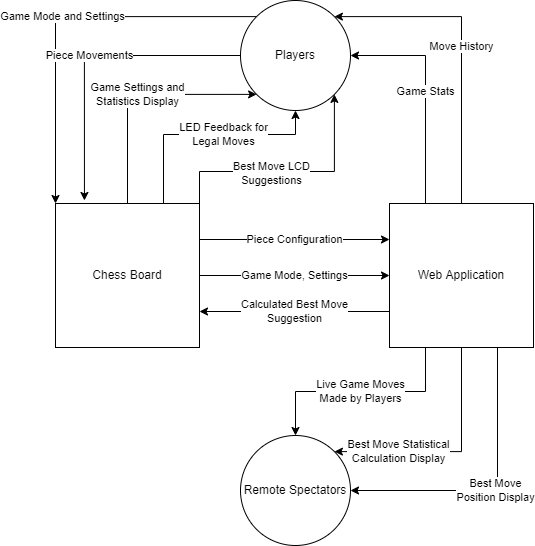
\includegraphics[scale=0.65]{chess-connect-system-context.png}
          \caption{Overall System Context}
          \label{Fig_SystemContext} 
        \end{center}
      \end{figure}
}

\section{Critical Assumptions}

The assumptions made in this document are meant to constrain the hazards to those present within typical operation. These assumptions are as follows:
\begin{enumerate}
    \item The chess board is operated in a dry environment.
    \item The server present will be capable of both Bluetooth and Wi-Fi connections.
    \item The user is not intentionally trying to disconnect the electronics within the board.
    \item The Web-App hosting platform will remain up and running without interruption.
\end{enumerate}

\section{Failure Modes and Effects Analysis}
{The failure modes and effects analysis is used to identify and analyze potential 
hazards to the system. Causes of failure discuss existing hazards that will have
negative effects on the system. Hazard detection details the methods used to distinguish
failures.Recommende actions explains the behavior of the system when the failures
occur. Likelihood is a scale to detail the frequency and probability-of-occurence
in the event of a failure. All of these methods are used to enhance requirement 
implementation and hazard prevention. \\

All prompts for user action will be displayed on the LCD embedded into the chess board.
Different prompts will correspond to different error screens, and different responses to the system.} 


\newgeometry{left=1cm,right=1cm,top=1cm,bottom=3cm}
\begin{center}
    \begin{longtable}{| >{\centering\arraybackslash}m{2.25cm} | 
        >{\centering\arraybackslash}m{2cm} | 
        >{\centering\arraybackslash}m{4cm} |
        >{\centering\arraybackslash}m{2cm} |
        >{\centering\arraybackslash}m{2.25cm} |
        >{\centering\arraybackslash}m{2cm}|
        >{\centering\arraybackslash}m{2cm}|}

    \caption{Failure Mode and Effects Analysis}\\

    \hline
    \rowcolor[gray]{0.9}
    Component & Failure & Causes & Detection & Recommended Action 
    & Likelihood & Requirements\\
    \hline

    Web Application & Loss of internet connection
    & \begin{enumerate}[label=(\alph*)]
        \item Internet outage
        \item Internet time-out 
        \item Board is taken out of connection range
    \end{enumerate} 
    & Ping the Internet and wait for the response 
    & Alert the user to check Internet connection 
    & 0.4 & SR3, SR4\\
    \hline

    Web Application & Connection lost between server and client
    & \begin{enumerate}[label=(\alph*)]
        \item Deployment hosting platform fails
        \item Platform is taken down for maintenance
    \end{enumerate} 
    & Loss of connection to the platform
    & Alert the user of the issue and wait accordingly
    & 0.1 & SR3, SR4\\
    \hline

    Microcontroller & Unable to detect starting game state &
    \begin{enumerate}[label=(\alph*)]
        \item A player begins with the pieces in the incorrect location
        \item Player does not follow the correct starting protocol
    \end{enumerate} 
    & Strict guidelines programmed in the microcontroller to prevent
    & Prompt user to make appropriate changes to pieces or board state
    & 0.2 & SR5\\ 
    \hline

    Microcontroller & Unable to follow game state &
    \begin{enumerate}[label=(\alph*)]
        \item A player makes two moves in a row
        \item A player makes an illegal move
        \item Loss of power to system
    \end{enumerate} 
    & Edge cases programmed on the controller
    & Prompt user to make appropriate action to the board
    & 0.3 & SR5\\ 
    \hline

    Microcontroller & Loss of Bluetooth connection & \begin{enumerate}[label=(\alph*)]
        \item Distance between microcontroller and host is too large
        \item Physical barriers between microcontroller and host
        \item Failed to initialise connection
        \item Packet loss from board to server
    \end{enumerate} 
    & Continuously monitor Bluetooth connection 
    & Prompt the user to re-establish connection before continuing 
    & 0.1 & SR3, SR4\\
    \hline

    Microcontroller & Loss of Power & \begin{enumerate}[label=(\alph*)]
        \item Board is unplugged
        \item Cable connection failure
        \item Power surge
    \end{enumerate} 
    & N/A
    & Store game state in local flash memory. Ensure proper electrical safety is adhered to (no exposed wires, solid connections, etc.)
    & 0.1 & SR3, SR8, SR9\\
    \hline

    Hall Sensor & Faulty sensor readings & \begin{enumerate}[label=(\alph*)]
        \item Sensitivity loss over a period of time
        \item Interference from external magnetic objects
        \item Distance between sensor and object too large
    \end{enumerate} & Monitoring Hall sensor inputs 
    & \begin{enumerate}[label=(\alph*)]
        \item Prompt the user to clear area of obstacles from the board
        \item The sensor should be replaced after the recommended use time
    \end{enumerate} 
    & 0.1 & SR5\\
    \hline

\end{longtable}
\end{center}
\restoregeometry

\newpage

\section{Safety and Security Requirements}

\subsection{Access Requirements}
\begin{enumerate}[{AC}1., leftmargin=2\parindent]
    \item Only the \progname{} team are able to modify the software system.
\end{enumerate}

\subsection{Integrity Requirements}
\begin{enumerate}[{IR}1., leftmargin=2\parindent]
    \item The product will not store game data after a game has concluded.
    \item The system shall locally maintain the current game state, making no changes until a connection is restablished.
    \item The system shall alert the user that a connection has been lost.
    \item The system shall prompt the user to take an appropriate hazard-specific action.
\end{enumerate}

\subsection{Privacy Requirements}
\begin{enumerate}[{PVR}1., leftmargin=2\parindent]
    \item The product will not store or collect user data.
\end{enumerate}

\subsection{Audit Requirements}
\begin{enumerate}[{AUR}1., leftmargin=2\parindent]
    \item Requirements shall be easy to follow and verify against both the system and the VnV (Verification and Validation) plan
        in order to facilitate regular inspections.
\end{enumerate}

\subsection{Safety Requirements}
\begin{enumerate}[{SR}1., leftmargin=2\parindent]
    \item The Arduino reuqires a 5V connection to power itself and all of the connected components. A laptop or a phone power adapter shall be plugged into a
        surge protector to ensure that power surges will not overload the system and cause damage or burns to the components.
    \item The wires, sensors and Arduino will be encapsulated within the wooden board so that the user has no access to any electrical components.
\end{enumerate}

\subsection{Immunity Requirements}
N/A

\section{Roadmap}

The hazard analysis has resulted in the development of more requirements related to the safety and security of the application. The hazard 
analysis also contains requirements that will be further specified in the VnV plan, allowing them to be verified according to specific 
fit criteria. This document will be frequently reviewed to recognize possible risks that can arise and reduce the likelihood of such
risks. Most of the requirements listed above will be applied to our project, while maintaining the possibility of not being able to 
implement some due to external factors such as project time constraints. Below is the planned roadmap of requirement implementation.

\textbf{Throughout the Course Term}
\begin{itemize}
    \item ACR1
    \item IR1
    \item IR2
    \item IR3
    \item IR4
    \item PVR1
\end{itemize}

\textbf{After the Completion of the Course Term}
\begin{itemize}
    \item AUR1
    \item SR1
    \item SR2
\end{itemize}

\newpage

\bibliographystyle {plainnat}
\bibliography {../../refs/References}
\end{document}
